\documentclass{beamer}\usepackage[]{graphicx}\usepackage[]{color}
%% maxwidth is the original width if it is less than linewidth
%% otherwise use linewidth (to make sure the graphics do not exceed the margin)
\makeatletter
\def\maxwidth{ %
  \ifdim\Gin@nat@width>\linewidth
    \linewidth
  \else
    \Gin@nat@width
  \fi
}
\makeatother

\definecolor{fgcolor}{rgb}{0.345, 0.345, 0.345}
\newcommand{\hlnum}[1]{\textcolor[rgb]{0.686,0.059,0.569}{#1}}%
\newcommand{\hlstr}[1]{\textcolor[rgb]{0.192,0.494,0.8}{#1}}%
\newcommand{\hlcom}[1]{\textcolor[rgb]{0.678,0.584,0.686}{\textit{#1}}}%
\newcommand{\hlopt}[1]{\textcolor[rgb]{0,0,0}{#1}}%
\newcommand{\hlstd}[1]{\textcolor[rgb]{0.345,0.345,0.345}{#1}}%
\newcommand{\hlkwa}[1]{\textcolor[rgb]{0.161,0.373,0.58}{\textbf{#1}}}%
\newcommand{\hlkwb}[1]{\textcolor[rgb]{0.69,0.353,0.396}{#1}}%
\newcommand{\hlkwc}[1]{\textcolor[rgb]{0.333,0.667,0.333}{#1}}%
\newcommand{\hlkwd}[1]{\textcolor[rgb]{0.737,0.353,0.396}{\textbf{#1}}}%

\usepackage{framed}
\makeatletter
\newenvironment{kframe}{%
 \def\at@end@of@kframe{}%
 \ifinner\ifhmode%
  \def\at@end@of@kframe{\end{minipage}}%
  \begin{minipage}{\columnwidth}%
 \fi\fi%
 \def\FrameCommand##1{\hskip\@totalleftmargin \hskip-\fboxsep
 \colorbox{shadecolor}{##1}\hskip-\fboxsep
     % There is no \\@totalrightmargin, so:
     \hskip-\linewidth \hskip-\@totalleftmargin \hskip\columnwidth}%
 \MakeFramed {\advance\hsize-\width
   \@totalleftmargin\z@ \linewidth\hsize
   \@setminipage}}%
 {\par\unskip\endMakeFramed%
 \at@end@of@kframe}
\makeatother

\definecolor{shadecolor}{rgb}{.97, .97, .97}
\definecolor{messagecolor}{rgb}{0, 0, 0}
\definecolor{warningcolor}{rgb}{1, 0, 1}
\definecolor{errorcolor}{rgb}{1, 0, 0}
\newenvironment{knitrout}{}{} % an empty environment to be redefined in TeX

\usepackage{alltt}            
\usepackage[english]{babel}
\usepackage[latin1]{inputenc}
\usepackage{graphicx}
\usepackage[T1]{fontenc}
\usepackage{lmodern}
\usepackage{caption}
\usepackage{booktabs}
\usepackage{textcomp}
\usepackage{epstopdf,tikz}
\usepackage{amsmath}

\usepackage[backend=biber, style=apa]{biblatex}
\DeclareLanguageMapping{american}{american-apa}

\usefonttheme[onlymath]{serif}

%%% defines highlight command to set text blue
\newcommand{\highlight}[1]{{\color{blue}{#1}}}
\addbibresource{bibliography.bib}

\usetheme{Boadilla}

\title{Feature-Label-Ordering}
\subtitle{a pre-registered Bayesian replication using MTurk}
\date{\today}
\author{Fabian Dablander \& Marcel Bechtold}
\institute{University of T\"{u}bingen}
\IfFileExists{upquote.sty}{\usepackage{upquote}}{}
\begin{document}

\begin{frame}
  \titlepage
\end{frame}

\begin{frame}
	\begin{quote}
		Gregory: ``Is there any other point to which you would wish to draw my attention?''\\
		Holmes: ``To the curious incident of the dog in the nighttime.''\\
		Gregoy: ``The dog did nothing in the nighttime.''\\
		Holmes: ``That was the curious incident.''\\
	\end{quote}
\end{frame}

\begin{frame}
	\begin{center}
		
\includegraphics[scale=0.7]{figure/meme.png}
	\end{center}
\end{frame}

\section{Introduction}
\begin{frame}{Error-driven learning}
    \begin{center}
        $V^{t+1}_{ij} = V^{t}_{ij} + \bigtriangleup V^t_{ij}$
    \end{center}
    
    \begin{small}
      \begin{equation*}
          \bigtriangleup V^t_{ij} = \begin{cases}
              0, & \text{if ABSENT($C_i$, t)} \\
              \alpha_i \beta_1(\lambda - \sum\nolimits_{\text{present{($C_j$, t)}}} V_{ij}), & \text{if PRESENT($C_j$, t) \& PRESENT(0, t)}\\
              \alpha_i \beta_2(0 - \sum\nolimits_{\text{present{($C_j$, t)}}} V_{ij}), & \text{if PRESENT($C_j$, t) \& ABSENT(0, t)}\\
             \end{cases}
      \end{equation*}
    \end{small}
\end{frame}

\begin{frame}{FL-learning vs. LF-learning\footnote{all images from Ramscar et al. (2010)}}
    \begin{center}
		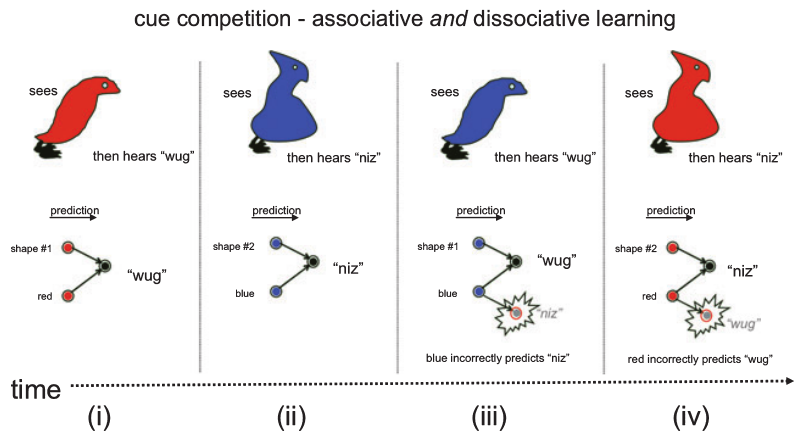
\includegraphics[scale=.4]{figure/FL_learning.png}
	\end{center}
\end{frame}

\begin{frame}{FL-learning vs. LF-learning}
    \begin{center}
    	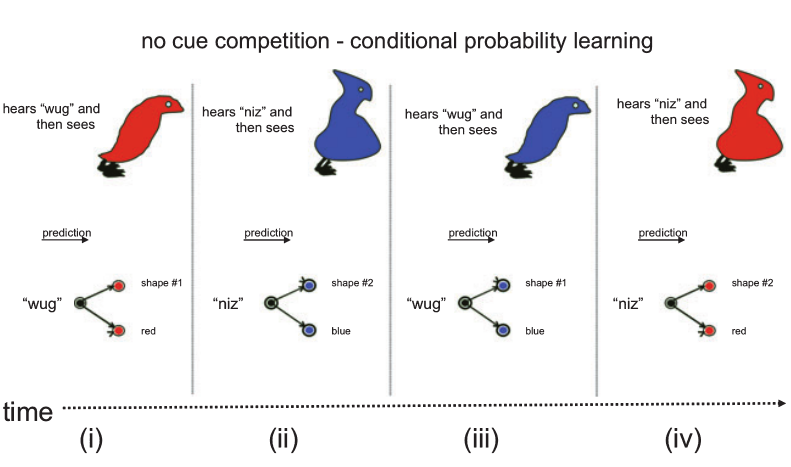
\includegraphics[scale=.4]{figure/LF_learning.png}
    \end{center}
\end{frame}

\begin{frame}{No representation without taxation (\cite{ramscar2009no})}
    \begin{center}
    	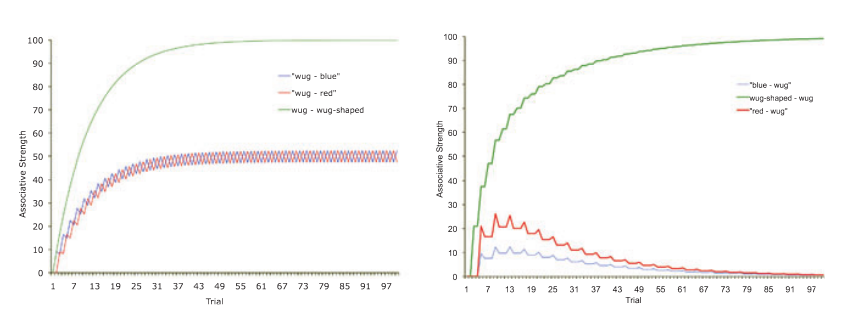
\includegraphics[scale=.4]{figure/representation.png}
    \end{center}
\end{frame}

\section{Design}
\begin{frame}{Example Trial\footnote{\href{http://wiki.cnbc.cmu.edu/Image_Databases}{great image databases: here}}}
    \begin{center}
        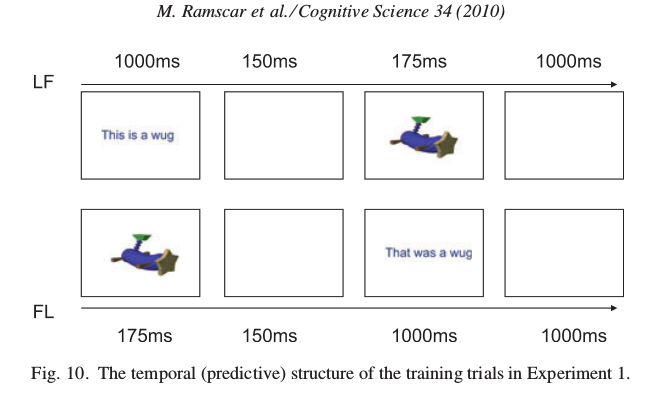
\includegraphics[scale=.45]{figure/trial.png}
	\end{center}
\end{frame}

\begin{frame}{Their Results}
    \begin{itemize}[<+->]
        \item All subjects were tested on a category verification and recognition task.
        \item A 2(learning) x 2(task) ANOVA found that training using FL-examples lead to better
              performance on the category verification task.
        \item Conversely, when trained on LF-examples, they scored higher on the recognition task.
        
        \item shows that \textbf{improved response-discrimination leads to the original input being less accurately represented}
    \end{itemize}
\end{frame}

\begin{frame}{Our Goal}
We want to replicate those results using an Amazon Mechanical Turk sample and using different statistical techniques.
\end{frame}

\section{Analysis}
\begin{frame}[fragile]{Bayesian Signal Detection Theory}
\begin{knitrout}
\definecolor{shadecolor}{rgb}{0.969, 0.969, 0.969}\color{fgcolor}\begin{kframe}
\begin{alltt}
\hlkwd{library}\hlstd{(}\hlstr{'rjags'}\hlstd{)}

\hlstd{ms} \hlkwb{<-} \hlstr{'
model \{
  hits ~ dbin(theta_h, signal)
  falarms ~ dbin(theta_f, noise)
    
  theta_h <- phi(d/2-c)
  theta_f <- phi(-d/2-c)
    
  d ~ dnorm(0, .5)
  c ~ dnorm(0, 2)
\}'}

\hlcom{# see also Lee & Wagenmakers (2013, pp.156)}
\end{alltt}
\end{kframe}
\end{knitrout}
\end{frame}

\begin{frame}[fragile]{Example}
\begin{knitrout}
\definecolor{shadecolor}{rgb}{0.969, 0.969, 0.969}\color{fgcolor}\begin{kframe}
\begin{alltt}
\hlkwd{library}\hlstd{(}\hlstr{'ggmcmc'}\hlstd{)}

\hlstd{params} \hlkwb{<-} \hlkwd{c}\hlstd{(}\hlstr{'d'}\hlstd{,} \hlstr{'c'}\hlstd{,} \hlstr{'theta_h'}\hlstd{,} \hlstr{'theta_f'}\hlstd{)}
\hlstd{data} \hlkwb{<-} \hlkwd{list}\hlstd{(}\hlstr{'hits'} \hlstd{=} \hlnum{70}\hlstd{,} \hlstr{'falarms'} \hlstd{=} \hlnum{50}\hlstd{,}
             \hlstr{'signal'} \hlstd{=} \hlnum{70} \hlopt{+} \hlnum{30}\hlstd{,} \hlstr{'noise'} \hlstd{=} \hlnum{50} \hlopt{+} \hlnum{50}\hlstd{)}

\hlstd{model} \hlkwb{<-} \hlkwd{jags.model}\hlstd{(}\hlkwd{textConnection}\hlstd{(ms),} \hlkwc{data} \hlstd{= data,}
                    \hlkwc{n.chains} \hlstd{=} \hlnum{2}\hlstd{,} \hlkwc{quiet} \hlstd{=} \hlnum{TRUE}\hlstd{)}

\hlstd{samples} \hlkwb{<-} \hlkwd{coda.samples}\hlstd{(model,} \hlkwc{n.iter} \hlstd{=} \hlnum{10000}\hlstd{,}
                        \hlkwc{variable.names} \hlstd{= params)}
\end{alltt}
\end{kframe}
\end{knitrout}
\end{frame}

\begin{frame}[fragile]{Example}
\begin{knitrout}
\definecolor{shadecolor}{rgb}{0.969, 0.969, 0.969}\color{fgcolor}\begin{kframe}
\begin{alltt}
\hlkwd{ggs_density}\hlstd{(}\hlkwd{ggs}\hlstd{(samples[,} \hlnum{1}\hlopt{:}\hlnum{2}\hlstd{]))}
\end{alltt}
\end{kframe}
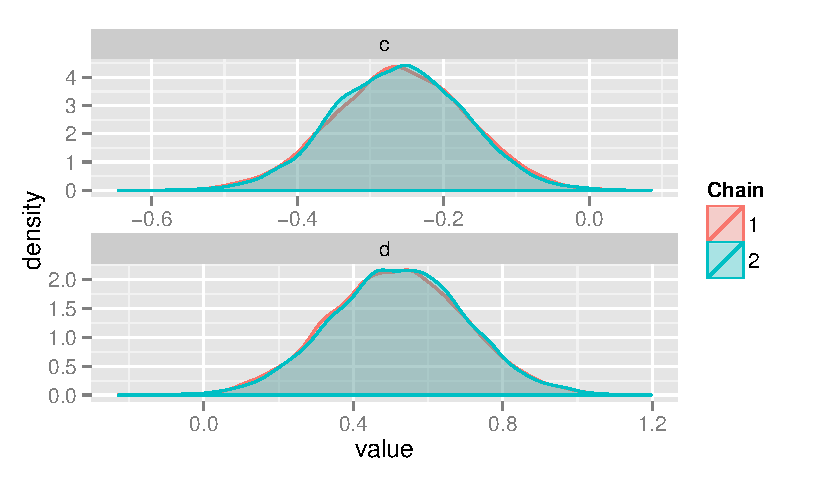
\includegraphics[width=\maxwidth]{figure/plot-1} 

\end{knitrout}
\end{frame}

\begin{frame}[fragile]{Mixed Logit Models}
Following \textcite{jaeger2008categorical}, \textcite{baayen2008mixed}, and \textcite{judd2012treating}, we want to analyze the gathered data
using a Mixed Logit Model with \emph{participant} and \emph{stimulus} as random factors.




\begin{knitrout}
\definecolor{shadecolor}{rgb}{0.969, 0.969, 0.969}\color{fgcolor}\begin{kframe}
\begin{alltt}
\hlkwd{library}\hlstd{(}\hlstr{'lme4'}\hlstd{)}

\hlcom{# example data}
\hlkwd{head}\hlstd{(data,} \hlnum{3}\hlstd{)}
\end{alltt}
\begin{verbatim}
##   id resp present cor alien learning         task
## 1  1    1       0   0   wug       FL  recognition
## 2  2    0       1   0   niz       FL verification
## 3  3    1       0   0   mob       LF  recognition
\end{verbatim}
\begin{alltt}
\hlcom{# example model}
\hlstd{fit} \hlkwb{<-} \hlkwd{glmer}\hlstd{(cor} \hlopt{~} \hlstd{learning}\hlopt{*}\hlstd{task} \hlopt{+} \hlstd{(}\hlnum{1}\hlopt{|}\hlstd{id)} \hlopt{+} \hlstd{(}\hlnum{1}\hlopt{|}\hlstd{alien),}
                   \hlstd{data, binomial)}
\end{alltt}
\end{kframe}
\end{knitrout}
\end{frame}

\section{Conclusion}
\begin{frame}{Plan}
    \begin{itemize}[<+->]
        \item pre-register replication on the \href{http://osf.io}{Open Science Framework}
        \item implement experiment in JavaScript, run it on Mechanical Turk
        \item implement Rescorla-Wagner simulations in R (Julia?)
        \item analyze data using Bayesian SDT and Mixed Logit Models
    \end{itemize}
\end{frame}

\end{document}
